% \textbf{\underline{OZ 6 - Magnetische inductie en de wet van Faraday - Oefening 3:}}
% \vspace{0.5cm}

% Een halfcirkelvormige geleider van straal $ R = 0,250 $ m wordt rondgedraaid rond de $ AC $-as in Figuur 6.3 met een constant tempo van 120 wentelingen per minuut. Een uniform magneetveld van 1,30 T wordt aangelegd in de regio net onder de staaf. Wat is de maximale geïnduceerde spanning in de geleider? Wat verandert er aan je antwoord als de staaf volledig in het magneetveld zou liggen? Teken het verloop van de geïnduceerde spanning in functie van de tijd voor beide gevallen.

% \begin{figure}[H]
%     \centering
%     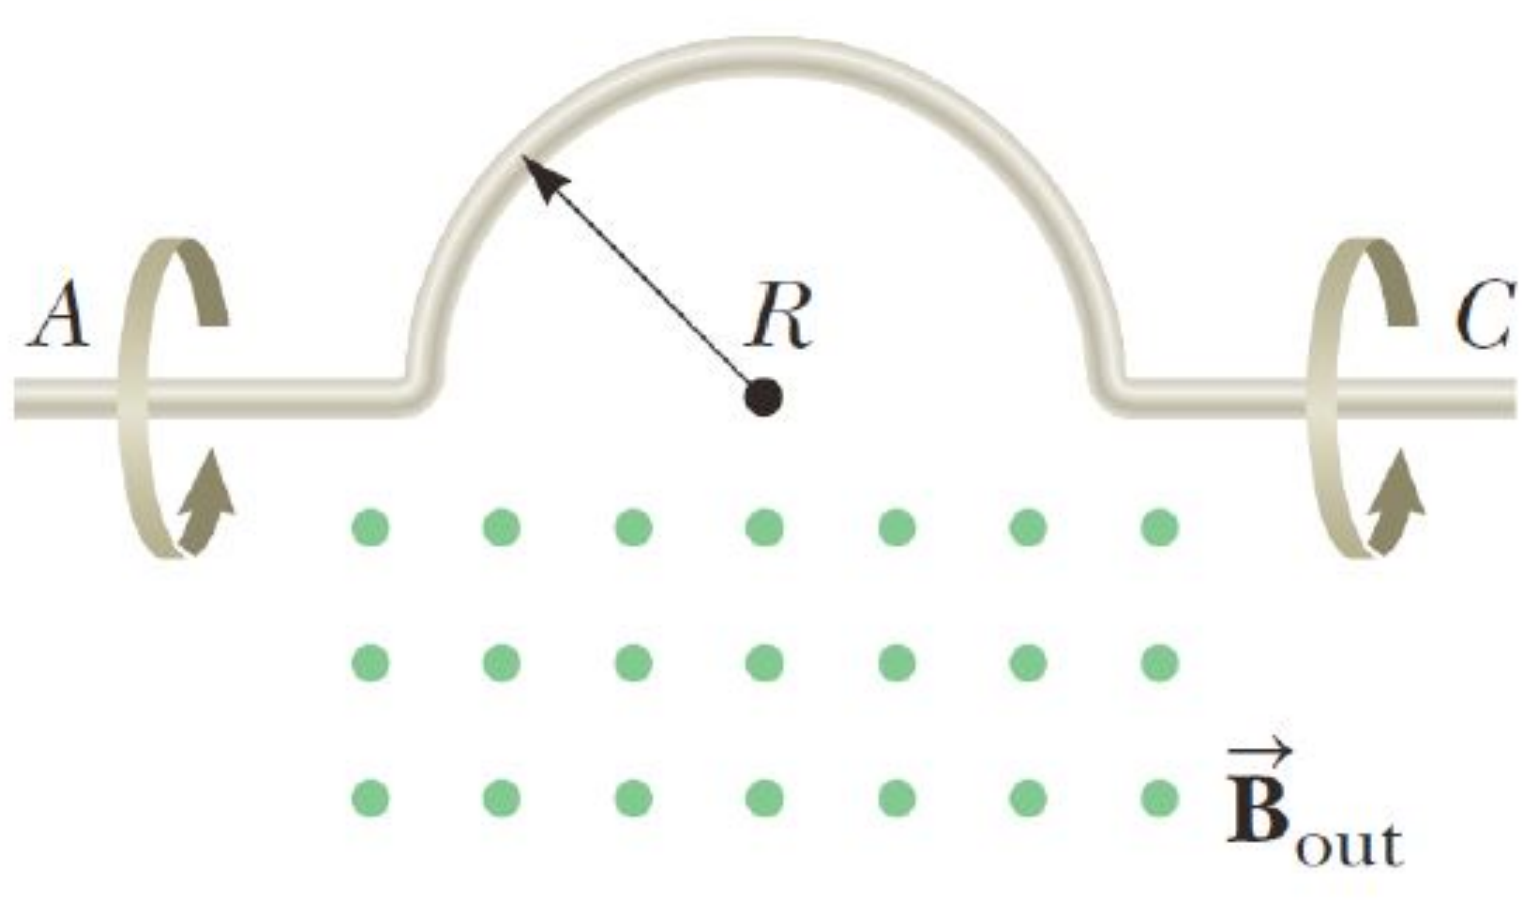
\includegraphics[width=6cm]{oz06/resources/oef-3-opgave.png}
    
%     \textbf{Figuur 6.3}
% \end{figure}

% \begin{description}[labelwidth=1.5cm, leftmargin=!]
%     \item[Geg. :]   $ R = 0,250 $ m; $ f = 120 $ min$ ^{-1} = 2 $ Hz; $ B = 1,30 $ T;
%     \item[Gevr. :]  $ \varepsilon_m $;
%     \item[Opl. :]   $ \omega = 2 \pi \cdot f $
    
%                     $ d\theta = \omega \ dt = 2 \pi \cdot f \ dt $
    
%                     \hspace{-0.57cm} $ \Rightarrow 
%                     \int_{0}^{\theta}{d\theta} = \int_{0}^{t}{2 \pi \cdot f \ dt} $
    
%                     \hspace{-0.57cm} $ \Rightarrow 
%                     \theta = 2 \pi \cdot f \cdot t $
                    
%                     \vspace{0.5cm}
                    
%                     In het veld:
%                     \begin{quote}
%                         $ \Phi_B = \int{\vec{B} \cdot d\vec{A}} 
%                         = B \cdot A \cdot \cos{\theta} 
%                         = B \cdot \dfrac{\pi \cdot R^2}{2} \cdot \cos{\left( 2 \pi \cdot f \cdot t \right)} $
                        
%                         $ \varepsilon = -\dfrac{d\Phi_B}{dt} 
%                         = B \cdot \pi^2 \cdot R^2 \cdot f \cdot \sin{\left( 2 \pi \cdot f \cdot t \right)} 
%                         = 1,30 \cdot \pi^2 \cdot 0,250^2 \cdot 2 \cdot \sin{\left( 4\pi \cdot t \right)} $
                        
%                         \hspace{0.15cm} $
%                         = 0,1625 \cdot \pi^2 \cdot \sin{\left( 4\pi \cdot t \right)} $
%                     \end{quote}
                    
%                     Niet in het veld: 
%                     \begin{quote}
%                         $ \Phi_B = \int{\vec{B} \cdot d\vec{A}} 
%                         = B \cdot A \cdot \cos{\theta} 
%                         = 0 \cdot \pi \cdot R^2 \cdot \cos{\left( 2 \pi \cdot f \cdot t \right)}
%                         = 0 $ Wb
                        
%                         $ \varepsilon = -\dfrac{d\Phi_B}{dt} 
%                         = 0 $
%                     \end{quote}
                    
%                     \vspace{0.5cm}
    
%                     $ \varepsilon = \left\{\begin{array}{ll}
%                         0,1625 \cdot \pi^2 \cdot \sin{\left( 4\pi \cdot t \right)} & \textrm{ als } t \in \left[ 0,125 + 0,5k; 0,375 + 0,5k \right]  \\
%                         0 & \textrm{ als } t \notin \left[ 0,125 + 0,5k; 0,375 + 0,5k \right]
%                     \end{array}\right. \textrm{ met } k \in \mathbb{Z} $
                    
%                     $ \varepsilon_{max} = 0,1625 \cdot \pi^2 = 1,60381 $ V $ \approx 1,60 $ V
                    
%                     \vspace{0.5cm}
                    
%                     Wanneer de staaf volledig in het veld ligt krijg je de volgende vergelijking:
                    
%                     \begin{quote}
%                         $ \varepsilon = 0,1625 \cdot \pi^2 \cdot \sin{\left( 4\pi \cdot t \right)} $
%                     \end{quote}
                    
%                     \begin{figure}[H]
%                         \centering
%                         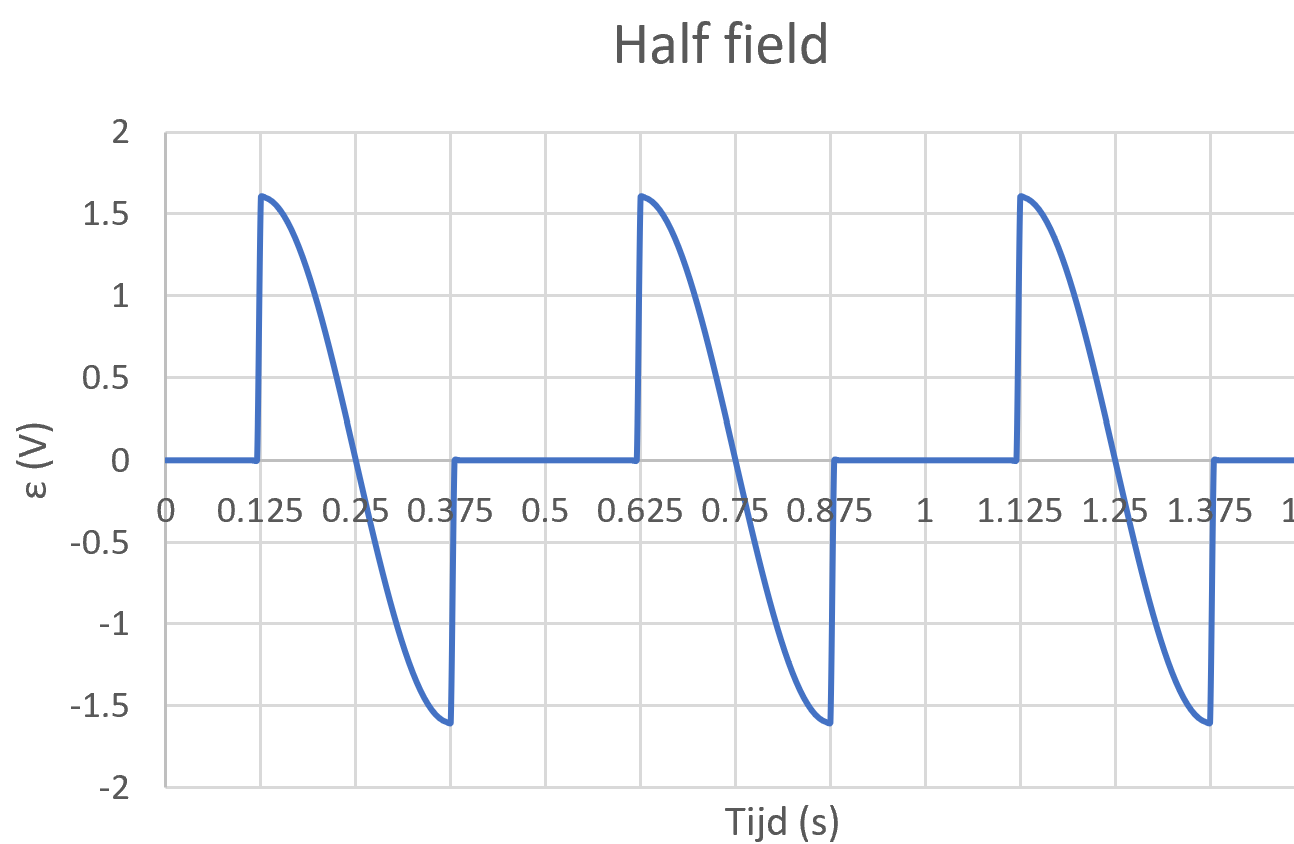
\includegraphics[width=10cm]{oz06/resources/oef-3-graph-1.png}
                        
%                         \textbf{Graph 6.1}
%                     \end{figure}
                    
%                     \begin{figure}[H]
%                         \centering
%                         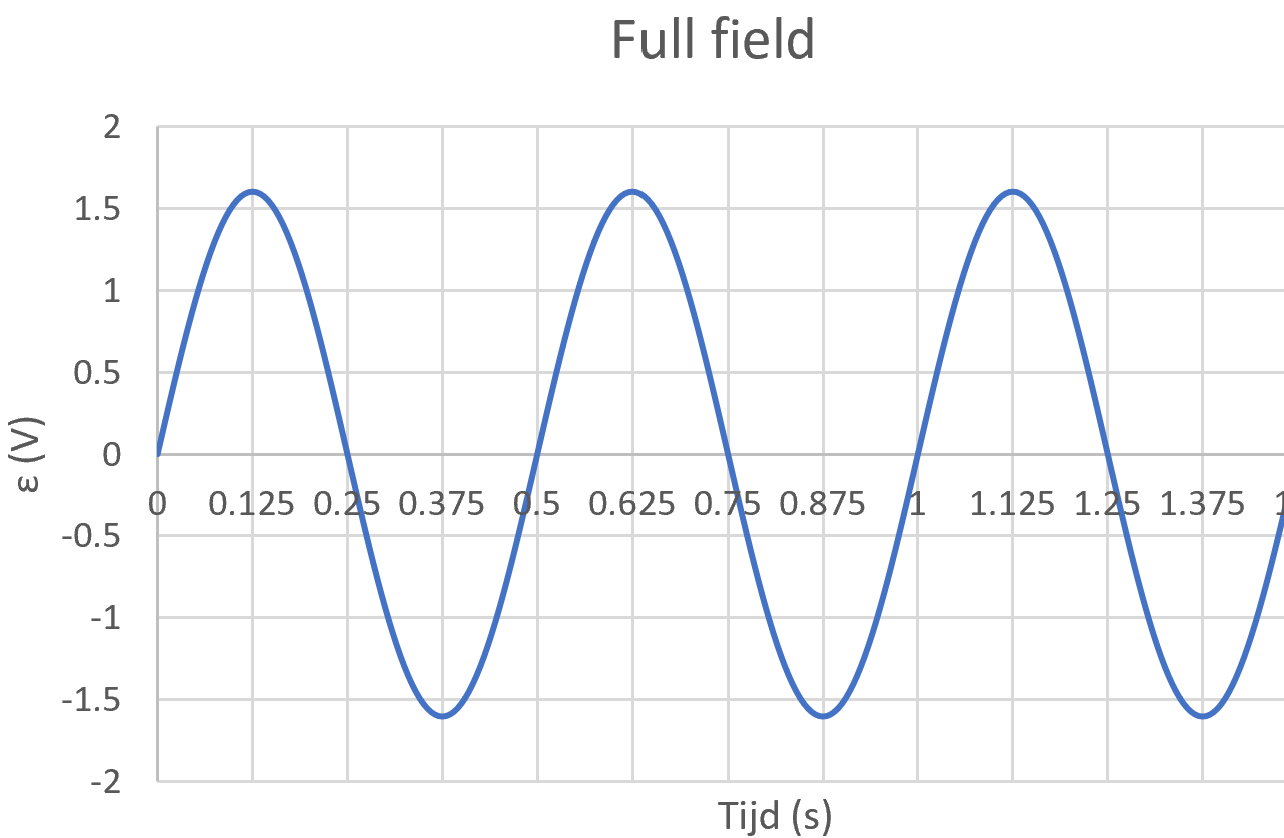
\includegraphics[width=10cm]{oz06/resources/oef-3-graph-2.png}
                        
%                         \textbf{Graph 6.2}
%                     \end{figure}
% \end{description}

% \vspace{1cm}